% ------------------------------------------------------------------------ %
% !TEX encoding = UTF-8
% !TEX TS-program = pdflatex
% !TEX root = ../Project.tex
% !TEX spellcheck = en-EN
% ------------------------------------------------------------------------ %
%
% ------------------------------------------------------------------------ %
% 	CHAPTER TITLE
% ------------------------------------------------------------------------ %
%
\chapter{Formal Analysis}
%
\label{cap:formalanalysis}
%
% ------------------------------------------------------------------------ %
%
\section{Modeling}
\lstinputlisting[language=alloy]{MainMatter/alloy.als}
%
% ------------------------------------------------------------------------ %
%
\begin{center}
\vspace{10mm}
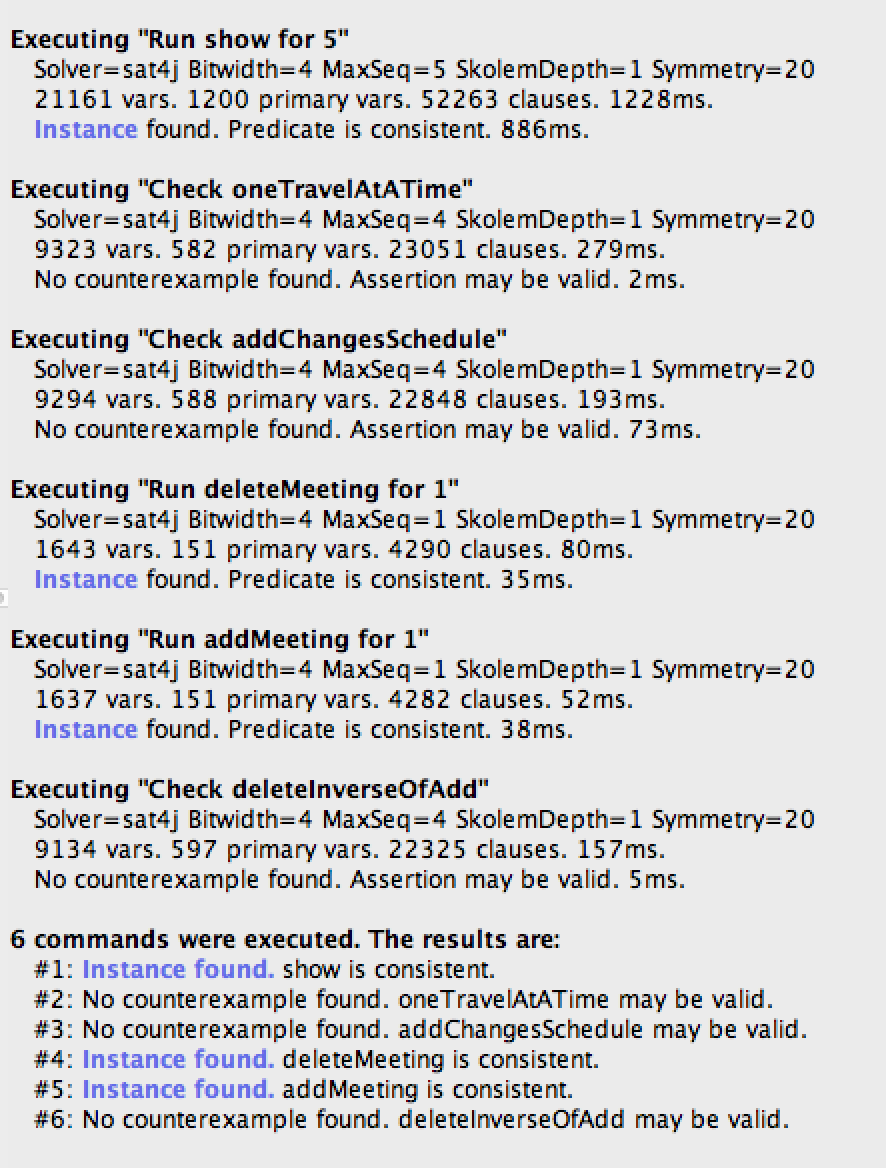
\includegraphics[scale=0.8]{MainMatter/images/alloy/results}
\captionof{figure}{Result of Alloy Analyzer}
\end{center}
%
\begin{landscape}
\section{World generated}
\begin{center}
\thispagestyle{empty}
\makebox[\textwidth][c]{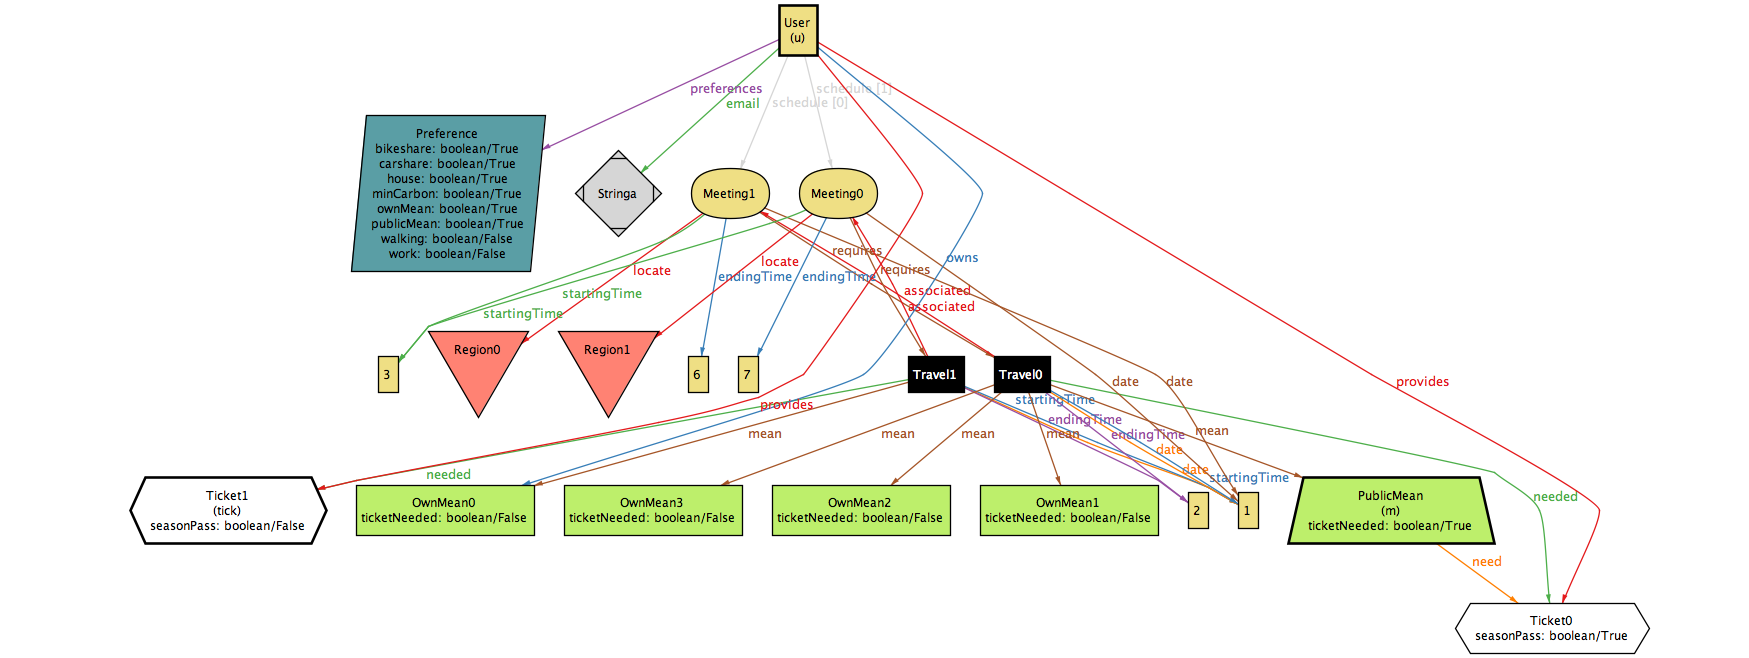
\includegraphics[width=2.3\textwidth]{MainMatter/images/alloy/world}}
\captionof{figure}{World generated}
\end{center}
\end{landscape}
%
\section{Alloy vs UML}
What we’ve modelled of the UML in alloy: \\
The goal of modelling in alloy is to describe some aspect of the system (but not the entire system), constrain it to exclude ill-formed examples and check properties about it.
The section in UML concerning the external companies connected to Travlendar+, for instance the ones which can provide tickets or that can offer sharing systems, is not modelled in Alloy cause we assume that they will behave correctly in our system thanks to the agreements they took with us.
We are also didn’t model time because it’s not useful in the model, but we will care about Time in other portions of the project analysis. The time break will not be modelled and also the fact that the application will not advise trips by bike or foot on late hours.
%
% -----------------------------END------------------------------------- %